\documentclass[12pt]{article}

\usepackage{sbc-template}
% \usepackage{hyperref}
\usepackage{graphicx,url}
\usepackage[brazil]{babel}
% \usepackage[latin1]{inputenc}
\usepackage{acro}
\usepackage[utf8]{inputenc}
\usepackage{amsmath,amssymb}
\usepackage{float}
\usepackage{xcolor}
\usepackage{booktabs}
\usepackage{tabularx}
\usepackage{svg}
\usepackage{pdfpages}

\pagestyle{plain} % Numeração centralizada no rodapé
\pagenumbering{arabic} % Formato 1, 2, 3...

\newcommand{\ric}[1]{\textcolor{magenta}{#1}}
\newcommand{\mth}[1]{\textcolor{red}{#1}}
\newcommand{\hide}[1]{}

\DeclareAcronym{ippuc}{
  short=Ippuc,
  long=Instituto de Pesquisa e Planejamento Urbano de Curitiba,
}

\DeclareAcronym{pois}{
  short=POIs,
  long=Pontos de Interesse,
}

\DeclareAcronym{idhm}{
  short=IDHM,
  long=Índice de Desenvolvimento Humano Municipal,
}

\DeclareAcronym{ipea}{
  short=Ipea,
  long=Instituto de Pesquisa Econômica Aplicada
}

\DeclareAcronym{ols}{
  short=MQO,
  long=Mínimos Quadrados Ordinários,
}

\DeclareAcronym{pca}{
  short=PCA,
  long=Análise de Componentes Principais,
}

\DeclareAcronym{ise}{
  short=ISE,
  long=indicadores socioeconômicos
}

\DeclareAcronym{PT}{
  short=PT,
  long=\textit{Proximity Time}
}

\DeclareAcronym{PTh}{
  short=PTh,
  long=Tempo de Acesso por Hexágono
}

\DeclareAcronym{SIG}{
  short=GIS,
  long=Geographic Information Systems
}

\sloppy
\title{A Framework for Assessing Short-Distance Urban Accessibility under Climate Disruptions}
%\title{Framework para Análise da Acessibilidade em Redes de Deslocamento sob Perturbações Climáticas}
%\title{Avaliação da Acessibilidade na Mobilidade de Curta Distância em Redes Urbanas sob Perturbações Climáticas}

\author{Matheus I. de Almeida\inst{1}, Ricardo Lüders\inst{1}, Luiz Gomes-Jr\inst{1}}


\address{Universidade Tecnológica Federal do Paraná (UTFPR)\\
  Curitiba -- PR -- Brazil
%\nextinstitute
%  Department of Computer Science -- University of Durham\\
%  Durham, U.K.
% \nextinstitute
%  Departamento de Sistemas e Computação\\
%  Universidade Regional de Blumenal (FURB) -- Blumenau, SC -- Brazil
  \email{matheusalmeida@alunos.utfpr.edu.br,\{luders,lcjunior\}@utfpr.edu.br}
}

\begin{document} 

\maketitle

\begin{abstract}
This work presents a framework for assessing short-distance accessibility under climate disruptions in the urban travel network. The city is modeled as a discrete spatial system composed of a grid of territorial units, a set of points of interest, and a travel network structured as a weighted graph. The framework estimates access times to everyday services under two scenarios: the typical network topology and a topology conditioned by environmental variables. In the conditioned scenario, edge weights are rewritten by a cost modifier that represents the effect of the environmental layer on mobility, admitting penalization, attenuation, or interdiction. The modifier handles continuous layers, such as land surface temperature, and discrete layers, such as geological risk polygons, and composes several layers either sequentially or jointly. Comparing the accessibility indicators obtained in the two scenarios, together with socioeconomic data, shows how the disruption alters access patterns and how the change distributes across the territory.

The framework is applied to two Brazilian state capitals, one carrying a continuous conditioning layer and the other discrete polygons. The comparison separates the loss of access from the increase in travel time, and a socioeconomic deprivation index built from three census variables locates the change within each city.
\end{abstract}
     
% \begin{resumo}
% Este trabalho propõe um framework para avaliação da acessibilidade de curta distância sob perturbações climáticas na rede urbana de deslocamentos. A cidade é modelada como um sistema espacial discreto composto por uma malha de unidades territoriais, um conjunto de pontos de interesse e uma rede de deslocamentos estruturada como um grafo ponderado. A partir dessa estrutura, são estimados tempos de acesso aos serviços cotidianos considerando dois cenários distintos: a topologia típica da rede de deslocamentos e uma topologia condicionada por variáveis ambientais. Neste último caso, os pesos das arestas do grafo são modificados por uma função de penalização que representa os efeitos das condicionantes climáticas sobre a mobilidade. A comparação entre os indicadores de acessibilidade obtidos nesses cenários, associada à integração de dados socioeconômicos, permite analisar como variáveis climáticas podem afetar os padrões de acessibilidade da população aos pontos de interesse urbanos e como esses impactos se distribuem espacialmente entre diferentes recortes populacionais.
% \end{resumo}

% \section{Introduction}

Active mobility — travel on foot, by bicycle, or by any means other than individually motorized vehicles — can help mitigate climate impacts. According to \cite{BRAND2021102764}, about 70\% of the life-cycle CO2 emissions per person from urban mobility activities come from cars, against only 1\% from bicycles. The authors estimate that each avoided car trip reduces individual emissions by 62\%.

Urban planning models have emerged in response to the climate emergency and to the search for decarbonization policies. One prominent model, currently being implemented in cities such as Paris and Barcelona, is the 15-minute city \cite{Allam2022-yx}. It organizes the city so that the services residents use daily are reachable through short trips, prioritizing active mobility.

The viability of such models depends on how the travel network behaves under real operating conditions. Prior work has shown that urban accessibility is not uniform: socioeconomic inequalities strongly shape who reaches which services and in what time \cite{sbbd_estendido}. Extreme climate events such as floods, intense rainfall, and landslides degrade mobility infrastructure, interrupting or obstructing segments of the road network and rendering certain trips unfeasible or substantially more costly. These disruptions do not affect the population evenly. Areas with higher vulnerability often show lower resilience to network degradation, and populations with less adaptive capacity bear larger impacts.

Answering these questions requires computing accessibility over heterogeneous spatial data. A city is described by a street graph, a set of points of interest, a discrete territorial grid, environmental rasters or polygons, and census aggregates, each with its own geometry, resolution, and coordinate reference system. Accessibility is then a many-to-many shortest-path problem whose cost function must absorb environmental evidence that is continuous in some cities and categorical in others. The computational problem is to make that pipeline reproducible and city-agnostic, so that the same analysis transfers to a new municipality by changing configuration rather than code.

This work evaluates how climate disruptions change urban accessibility and how those impacts are distributed unevenly across space and socioeconomic profiles. We propose a methodological approach that integrates travel-network modeling with socioeconomic analysis and compares typical scenarios (without disruption) against scenarios conditioned by environmental variables. The approach is implemented as an open-source library with a declarative workflow, in which penalty functions, data layers, and scenario definitions are configured rather than hard-coded.

The contributions of this work are threefold:

\begin{itemize}
  \item an open computational framework for modeling urban accessibility under environmental disruption, whose region-agnostic data model and declarative scenario configuration allow the same pipeline to be applied to different cities;
  \item a comparison of scenarios that distinguishes access loss from travel time increase, producing quantitative evidence on two Brazilian state capitals under different climate stressors;
  \item an assessment of how accessibility degradation correlates with socioeconomic conditions, exposing which populations bear the largest impacts.
\end{itemize}

The remainder of this paper is organized as follows. Section~\ref{sec:fundamentals} reviews the concepts of urban accessibility, active mobility, and environmental disruption. Section~\ref{sec:methodology} presents the framework and its penalization mechanism, and Section~\ref{sec:case_studies} describes the two case studies and their calibration. Section~\ref{sec:results} reports the results. Section~\ref{sec:discussion} discusses limitations and implications, and Section~\ref{sec:conclusion} concludes.

% \input{sections/2.related_work}
% \section{Methodology}
\label{sec:methodology}

This section presents the methodology for assessing how environmental and climate disruptions reduce urban accessibility and affect different social groups. The method compares two states of the travel network: one under typical conditions and one modified by environmental variables. Holding the territory, the opportunities, and the indicator set fixed, the difference between them isolates and quantifies the loss of access caused by the disruption.

Section~\ref{sec:architecture} describes the framework architecture and its data model, Section~\ref{sec:penalization} details the penalization mechanism that rewrites network costs from environmental evidence, and Section~\ref{subsec:applicability} states the criterion by which the scenarios used in the case studies were selected.

\subsection{Framework Architecture}
\label{sec:architecture}

The framework separates \emph{what} is modeled from \emph{how} a specific city supplies it. A common computational core defines the territorial model, the routing procedure, and the indicator set, while everything that varies across municipalities — data paths, penalty parameters, and scenario composition — is declared in configuration. The core is organized into modules with distinct responsibilities: \texttt{grid} and \texttt{network} build the spatial support, \texttt{pois} and \texttt{environment} load destinations and environmental layers, \texttt{penalties} rewrites edge costs, \texttt{routing} computes distance matrices, and \texttt{demographics} and \texttt{indicators} produce the socioeconomic and accessibility measures. A new city requires no change to these modules, only a new configuration file, and the comparison between a typical and a conditioned scenario follows from the same implementation.

Figure~\ref{fig:framework} summarizes the flow. The left panel shows the network under the typical scenario, with its original travel costs. The central panel shows the penalization mechanism, which uses environmental data to rewrite the cost of the mobility infrastructure. The right panel shows the conditioned scenario, where longer edges represent the added time or cost caused by the disruption.

\begin{figure}[H]
  \centering
  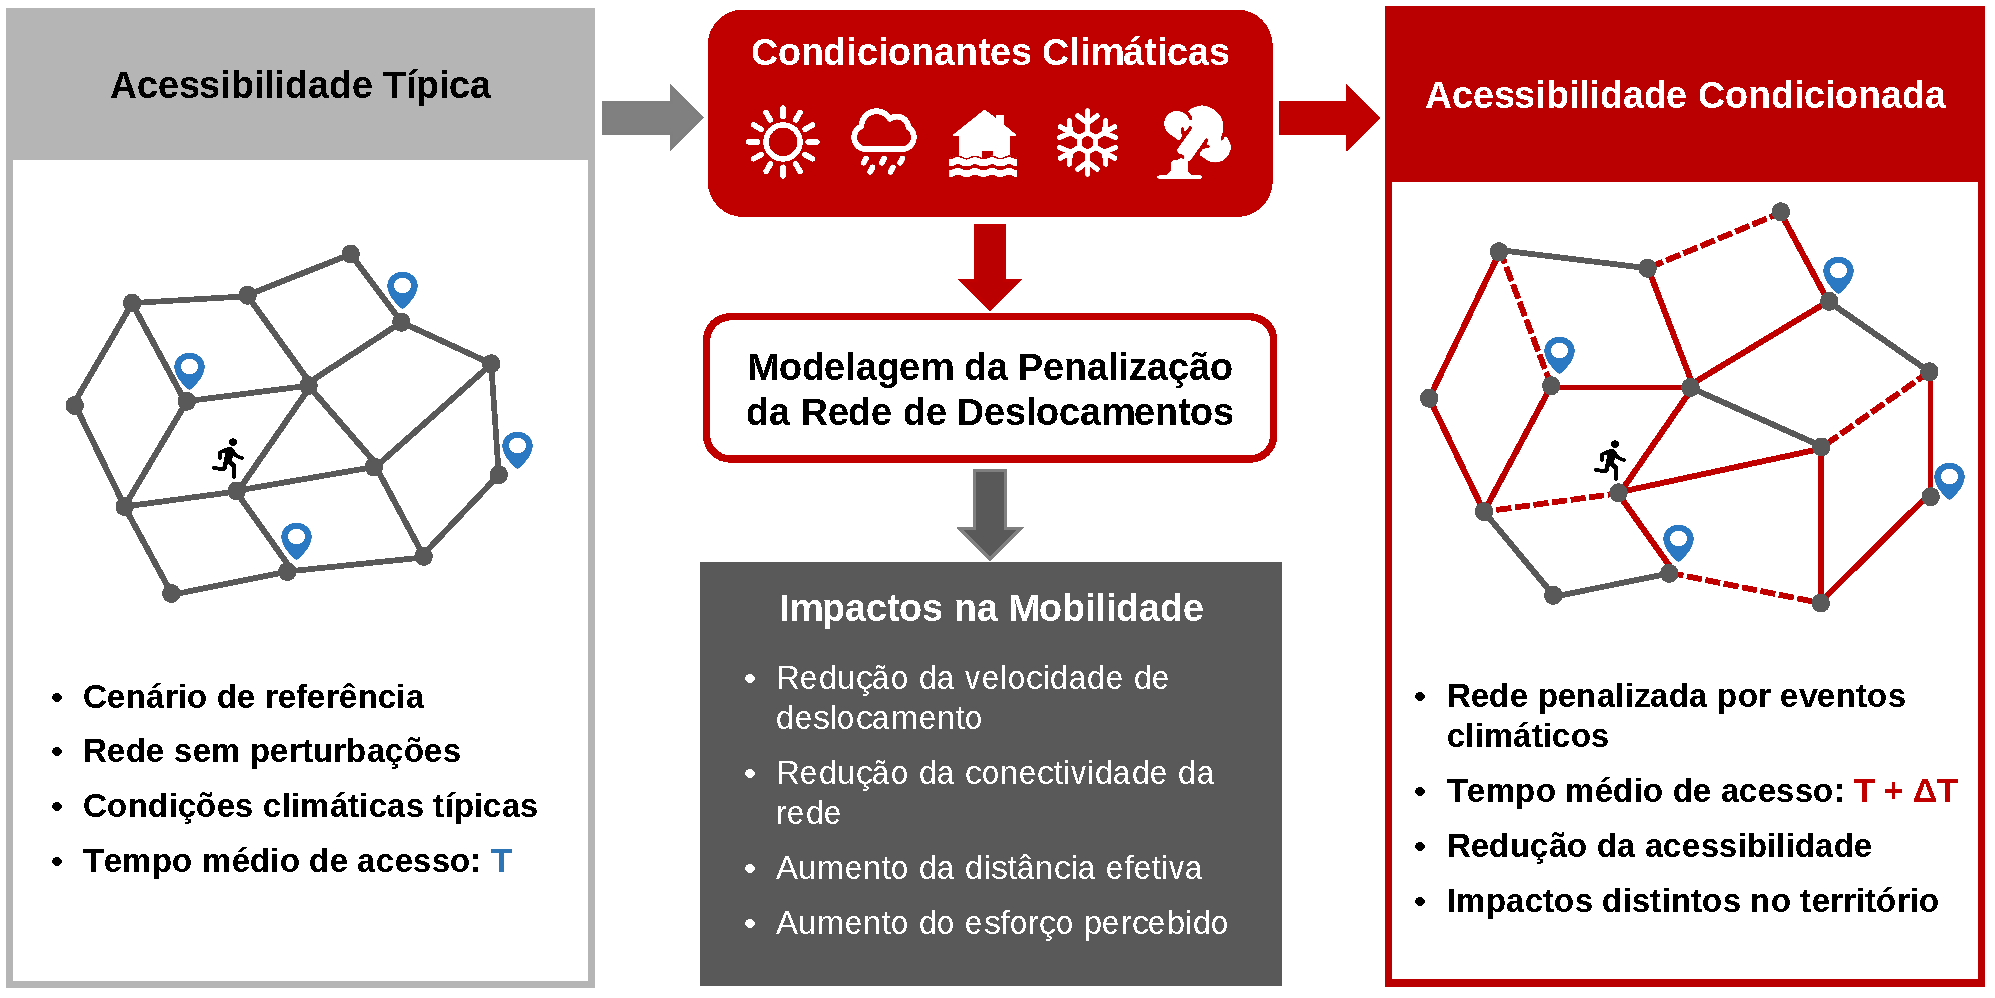
\includegraphics[width=1\textwidth]{figs/framework.pdf}
  \caption{Modeling flow for accessibility scenarios. Edges lengthen as their travel cost increases, so the geometry in the right panel encodes the effect of the disruption rather than the physical street layout.}
  \label{fig:framework}
\end{figure}

\subsubsection{Territorial Modeling}
\label{subsec:territorial_modelling}

The urban territory is assembled from four data types that differ in geometry, resolution, and coordinate reference system, and whose integration is the first source of complexity in the pipeline.

\begin{description}
  \item[Analysis grid.] A regular partition of the territory defining the minimum unit of study. The library supports hexagonal and square cells; the side or radius is a parameter set according to the transport mode and the local context. With hexagonal cells, the distance between neighboring centroids is uniform in all six directions, which avoids the directional bias that square cells introduce in neighborhood-based aggregation. The centroid of each cell is the theoretical origin of trips and the basis for computing and aggregating indicators.
  \item[Points of interest (POIs).] The destinations of trips: coordinates locating the everyday services used by the population, organized into categories such as health, education, and transport. Their selection depends on the availability of local databases, whether official or crowdsourced. Each POI is snapped to the nearest network vertex before routing, so the reachable set is bounded by the network rather than by straight-line distance.
  \item[Street network.] The mobility infrastructure is structured as a spatial graph, with vertices at intersections and edges along street segments whose initial base weight is travel time. Each cell centroid is attached to the nearest network vertex, and a maximum snap distance discards cells whose centroid lies too far from the network — a parameter that prevents a cell in an unmapped area from being routed through a vertex several kilometers away. Because this threshold removes cells from the analysis, it must be reported alongside the results.
  \item[Environmental layers.] Spatial layers that may be continuous, such as raster images, or discrete, such as vector polygons, mapping the climate or environmental phenomena under evaluation. A single scenario may stack several such layers. They are overlaid on the street network to adjust the travel cost of affected edges, as described in Section~\ref{sec:penalization}.
\end{description}

A fifth input completes the model. \textbf{Demographic and socioeconomic data} characterize the resident population — density, income, and schooling — and come from official censuses. These data are published in irregular administrative units such as census tracts, which do not align with the analysis grid, so each tract attribute is transferred to the cells by area-weighted mean: a cell receives the average of the tract values covering it, weighted by the intersected area. Where a tract has no value, its area is excluded from the denominator, so a cell partially covered by suppressed data is not diluted toward zero. The numerator and denominator are both taken from tracts with data, which keeps the cell value equal to the value of its contributing tracts rather than to a fraction of it.

This distinction between interpolation by density and aggregation by area is not interchangeable. Density interpolation conserves totals and suits population counts; area-weighted averaging preserves the value of the attribute itself and suits rates and indices. Population is interpolated the first way, socioeconomic indices the second.

\subsection{The Cost-Modification Mechanism}
\label{sec:penalization}

The framework fixes neither which environmental variables alter the network nor the magnitude of their effect. It exposes a \emph{mechanism} that receives environmental layers and returns a new cost for each edge; selecting the layers and setting their parameters belongs to whoever applies the method. This section describes that mechanism.

\subsubsection{Scenarios}

The network is evaluated in two states. In the \textbf{typical scenario}, each edge weight ($W_{base}$) is the travel cost under normal conditions — the segment length divided by the mean speed adopted for the mode under analysis. In the \textbf{conditioned scenario}, weights are recomputed from the environmental layers ($C$), producing $W_{cond}$ for each edge.

Comparing the two states isolates the effect of the disruption: any difference in accessibility indicators is attributed to the cost change introduced by the environmental layers.

\subsubsection{Cost modifiers}

The core element of the mechanism is the \emph{cost modifier}. Each modifier is a function that takes the value of a layer at a point on the edge and returns a multiplicative factor:

\begin{equation}
  f(v) \rightarrow \mathbb{R}^{+}
\end{equation}

where $v$ is the value sampled from the layer at that point. The factor $f$ may exceed 1 (penalization), fall below 1 (attenuation), or be infinite (interdiction). The same mechanism covers all three cases, which is why the framework refers to \emph{cost modifiers} rather than penalties alone.

A modifier never receives the whole edge: it is applied to values sampled along it. Sampling strategy and factor aggregation are declared separately, so phenomena with different spatial distributions are handled by the same mechanism.

\subsubsection{Sampling}

Two sampling strategies are available, and the choice trades cost for fidelity. \textbf{Midpoint} queries the layer at the edge midpoint and applies a single factor to the entire edge, which is fast but inaccurate when the edge crosses a boundary. \textbf{Segments} places $n$ equidistant points along the edge, including both endpoints, and reads the layer at each; the value of $n$ is a parameter, defaulting to four.

The distinction matters most for long edges, which are common in peripheries where blocks are large. A single edge can span several hundred meters and cross more than one thermal or topographic zone. Sampling only its midpoint may place the entire segment in the wrong class.

\subsubsection{Reading the layers}

How a layer is queried depends on the nature of the data.

\textbf{Continuous data} (rasters) are sampled at the chosen points. Each point takes the value of the pixel containing it. Points landing on a nodata pixel leave the cost unchanged at that location rather than propagating a missing value into the cost, so an incomplete raster degrades coverage instead of corrupting the network.

\textbf{Discrete data} (vector polygons) are queried by intersection. The edge is partitioned at every point where a polygon boundary crosses it, and each resulting sub-segment receives the factor of the polygon covering it. Sub-segments outside any polygon keep the original cost. Where polygons overlap, the \emph{largest} factor among them applies to the overlap, so a region mapped by two hazard layers is governed by the more restrictive one.

\subsubsection{Aggregation and interdiction}

The factors obtained along an edge must be reduced to a single value for the whole edge. The framework offers two reductions:

\begin{itemize}
  \item \textbf{Maximum}: adopts the most restrictive factor observed along the segment, treating the edge by its worst case. This is conservative and appropriate when the sample is small.
  \item \textbf{Length-weighted mean}: each sub-segment pays its own factor, and the mean is weighted by extent. This is more faithful on long edges crossing heterogeneous regions.
\end{itemize}

Infinite factors receive separate treatment. Assigning $f = \infty$ to a sub-segment declares it impassable: the cost of any path crossing it becomes infinite, and routing prefers alternatives. Interdiction is not a high cost but a statement that crossing is not viable in that scenario — the appropriate treatment for phenomena that block the road rather than delay it, such as a landslide burying the segment. When no alternative exists, the cell reaches no destination at all, a situation recorded as access loss.

\subsubsection{Composition}

When more than one environmental layer affects the same edge, modifiers are applied in sequence and the result accumulates multiplicatively:

\begin{equation}
  W_{cond} = W_{base} \times f_1 \times f_2 \times \cdots \times f_n
\end{equation}

Each step receives the cost produced by the previous one. Because multiplication commutes, the order does not change the numeric result, but it changes how the process reads, which matters when attributing an accessibility change to a specific layer.

This composition admits two arrangements. In \emph{simple rules}, each modifier queries one layer independently and chaining happens across rules. In \emph{composite rules}, several layers are queried at the same point on the edge and the factor is computed jointly, allowing one layer's effect to depend on another's value.

The distinction is not cosmetic. In the simple arrangement, an attenuation by vegetation would apply to any tree-lined segment, including where there is no heat at all — dense canopy next to a shaded, cool street would still receive a discount. In the composite arrangement, vegetation attenuates only where the thermal layer exceeds a threshold at that same point, so the two factors are evaluated jointly rather than independently averaged. A composite rule thus samples all its layers at identical locations before aggregating, preserving the spatial correspondence between their values.

\subsubsection{Recalculation and indicators}

With conditioned costs defined, a least-cost path algorithm runs over the graph, producing travel-time matrices for both scenarios. From these, the indicators described in Section~\ref{subsec:territorial_modelling} are computed: the mean time to reach the $k$ nearest POIs of each category (PTh), the inequality of its distribution (index G), and the share of the population served within a threshold (F15).

The scenario comparison adds per-cell time variation and \emph{access loss}: cells reaching no POI under the conditioned scenario receive infinite time and are accounted for separately. They are not an extreme case of high time but the absence of access, and treating them as a numeric value would distort any mean or inequality index computed over the remainder.

\subsection{Applicability}
\label{subsec:applicability}

This section states the criterion by which the scenarios were selected. The mechanism must handle environmental evidence in several forms, and each scenario instantiates one of them.

\subsubsection{Selection Criterion}

The mechanism varies along three axes: whether the environmental layer is continuous or discrete, whether several layers are read independently or jointly at the same location, and whether the effect is a penalization or an interdiction. Each scenario instantiates one combination of these values, and the set was chosen so that each axis appears at both of its values.

Several scenarios run on the same city and differ only in the layers they declare, so the variation in behavior follows from configuration.

\subsubsection{Coverage of the Mechanism}

Table~\ref{tab:cenarios} lists the seven conditioned scenarios by the capability each exercises.

\begin{table}[H]
\centering
\footnotesize
\caption{Scenarios by the capability of the mechanism they exercise}
\label{tab:cenarios}
\begin{tabularx}{\linewidth}{|l|l|X|l|}
\hline
\textbf{Scenario} & \textbf{Layers} & \textbf{Capability exercised} & \textbf{Effect} \\
\hline
\texttt{thermal} & 1 raster & Sampling of a continuous field & penalization \\
\texttt{thermal+green} & 2 rasters, joint & Composite rule over co-located layers & penalization \\
\texttt{thermal\_demo} & 1 raster & Response to a steeper gradient & penalization \\
\texttt{thermal+green\_demo} & 2 rasters, joint & Composite rule under a steeper gradient & penalization \\
\texttt{flood} & 1 vector & Partition at polygon boundaries & penalization \\
\texttt{landslide} & 1 vector & Same, with infinite factors & interdiction \\
\texttt{flood+landslide} & 2 vectors & Sequential composition, interdiction dominates & both \\
\hline
\end{tabularx}
\end{table}

Three properties follow from the table.

\textbf{Both branches of the modifier are exercised.} Curitiba samples continuous fields and Porto Alegre intersects polygon geometries, which are distinct implementation paths.

\textbf{Both outcomes of the cost function are exercised.} Flooding raises travel cost while preserving every connection, so all paths exist in both scenarios with a different weight. Landsliding makes segments impassable, and some origins lose access entirely. The framework reports the second separately, since it is an absence of access and not a slowdown.

\textbf{Composition appears in homogeneous and sequential form.} The \texttt{thermal+green} scenario reads two rasters at identical sampled points and returns a single factor, the thermal one multiplied by the shading reduction wherever vegetation is present. Sampling both layers at the same position is what requires a composite rule: two chained simple rules would each sample the segment independently and could read vegetation at a point whose temperature was read elsewhere. The \texttt{flood+landslide} scenario applies two vector rules in sequence, and the interdiction of one dominates the penalization of the other on shared edges.

\subsubsection{Demonstrative Scenarios}

Two Curitiba scenarios use a thermal coefficient roughly seven times the calibrated value. They are demonstrative, and the text does not read them as estimates. Their purpose is to show that the mechanism responds monotonically to the magnitude of its input: a steeper gradient that produced a smaller accessibility change would indicate a defect in the composition. Reporting them alongside the calibrated scenarios makes the sensitivity of the pipeline observable at no additional cost, since they differ only in a parameter.
\subsubsection{Scope and Limitations}

Two limits follow from the design and belong alongside the results.

\textbf{The mixed representation is supported at the component level.} The implementation reads a raster and a vector at the same sample point, and tests cover this path, but no scenario here declares one of each. Doing so requires a study area where both evidence types describe the same phenomenon, which the two municipalities do not provide.

\textbf{The estimates await validation against observations.} Accessibility under a hypothetical disruption has no measured counterpart, since the conditioned scenario did not occur. This work establishes that the mechanism computes what it specifies and that the framework accommodates disruptions of different forms. Matching the resulting travel times to what pedestrians would experience requires observed mobility under an actual event.

Together these limits place the contribution: a framework demonstrated to be applicable across representations and outcomes. Empirical validation of its predictions remains open.


% \input{sections/4.results}
% \input{sections/5.considerations}

\section{Introduction}

Active mobility — travel on foot, by bicycle, or by any means other than individually motorized vehicles — can help mitigate climate impacts. According to \cite{BRAND2021102764}, about 70\% of the life-cycle CO2 emissions per person from urban mobility activities come from cars, against only 1\% from bicycles. The authors estimate that each avoided car trip reduces individual emissions by 62\%.

Urban planning models have emerged in response to the climate emergency and to the search for decarbonization policies. One prominent model, currently being implemented in cities such as Paris and Barcelona, is the 15-minute city \cite{Allam2022-yx}. It organizes the city so that the services residents use daily are reachable through short trips, prioritizing active mobility.

The viability of such models depends on how the travel network behaves under real operating conditions. Prior work has shown that urban accessibility is not uniform: socioeconomic inequalities strongly shape who reaches which services and in what time \cite{sbbd_estendido}. Extreme climate events such as floods, intense rainfall, and landslides degrade mobility infrastructure, interrupting or obstructing segments of the road network and rendering certain trips unfeasible or substantially more costly. These disruptions do not affect the population evenly. Areas with higher vulnerability often show lower resilience to network degradation, and populations with less adaptive capacity bear larger impacts.

Answering these questions requires computing accessibility over heterogeneous spatial data. A city is described by a street graph, a set of points of interest, a discrete territorial grid, environmental rasters or polygons, and census aggregates, each with its own geometry, resolution, and coordinate reference system. Accessibility is then a many-to-many shortest-path problem whose cost function must absorb environmental evidence that is continuous in some cities and categorical in others. The computational problem is to make that pipeline reproducible and city-agnostic, so that the same analysis transfers to a new municipality by changing configuration rather than code.

This work evaluates how climate disruptions change urban accessibility and how those impacts are distributed unevenly across space and socioeconomic profiles. We propose a methodological approach that integrates travel-network modeling with socioeconomic analysis and compares typical scenarios (without disruption) against scenarios conditioned by environmental variables. The approach is implemented as an open-source library with a declarative workflow, in which penalty functions, data layers, and scenario definitions are configured rather than hard-coded.

The contributions of this work are threefold:

\begin{itemize}
  \item an open computational framework for modeling urban accessibility under environmental disruption, whose region-agnostic data model and declarative scenario configuration allow the same pipeline to be applied to different cities;
  \item a comparison of scenarios that distinguishes access loss from travel time increase, producing quantitative evidence on two Brazilian state capitals under different climate stressors;
  \item an assessment of how accessibility degradation correlates with socioeconomic conditions, exposing which populations bear the largest impacts.
\end{itemize}

The remainder of this paper is organized as follows. Section~\ref{sec:fundamentals} reviews the concepts of urban accessibility, active mobility, and environmental disruption. Section~\ref{sec:methodology} presents the framework and its penalization mechanism, and Section~\ref{sec:case_studies} describes the two case studies and their calibration. Section~\ref{sec:results} reports the results. Section~\ref{sec:discussion} discusses limitations and implications, and Section~\ref{sec:conclusion} concludes.

\section{Fundamentals and Related Work}
\label{sec:fundamentals}

This section defines urban accessibility, describes how it is computed over a travel network, and reviews the literature on accessibility under environmental disruption and on spatial inequality.

\subsection{Urban Accessibility}

In urban and transport studies, urban accessibility describes how easily opportunities — services, jobs, facilities, and activities — can be reached from an origin. Unlike mobility, which is observed movement, accessibility is a structural property of the urban system: it depends on where opportunities are located, on how the network connects origins and destinations, and on which impedances (costs) are imposed on travel~\cite{Handy1997Measuring}. Accessibility is therefore usually treated as a measure of access potential rather than a direct measure of realized trips.

Formally, the territory is represented by a set of origins $O$ — territorial cells, tract centroids, blocks, or residence points — and a set of destinations $D$ (points of interest, POIs). A cost function $c(o,d)$ assigns to each pair $(o,d)$ the minimum travel cost between $o \in O$ and $d \in D$~\cite{Miller1999Measuring}. In network-based applications this cost is typically obtained by shortest-path algorithms over a travel graph, using walking or cycling time, and it provides the basis for indicators that are comparable across areas and scenarios.

Although often expressed as time or distance, $c(o,d)$ is better understood as a composite impedance that also captures comfort, safety, physical effort, and route reliability~\cite{Puello2016Integration}. This matters for short-distance active mobility~\cite{Cook2022More}, where the experience of the route and local conditions — slope, crossings, sidewalk quality, exposure to sun, rain, or wind, and the presence of flooding — can alter the viability of a trip even when the network geometry is unchanged. Climate disruptions can thus enter the problem as changes to the generalized travel cost, rather than only as binary segment closures.

Within location-based accessibility measures, reviews such as \cite{Geurs2004} group indicators by their assumptions: distance or minimum-cost measures, cumulative (contour) measures, and potential (gravity) measures. These families differ in how they treat destination choice, substitutability among opportunities, and distance or time decay, yet they share the premise that accessibility is derived from an origin-destination cost matrix.

The simplest measures are distance metrics, in which the accessibility of an origin is the minimum cost to the nearest opportunity — for example, the time to the nearest shop. Such an indicator is intuitive and adequate when users are assumed to satisfy a need at the easiest destination to reach. It ignores the existence of multiple alternatives, does not represent competition among offers, and can be unstable when small network changes alter which POI is nearest.

When the availability of multiple opportunities matters, cumulative (contour) measures count how many opportunities are reachable within a cost threshold, such as the number of POIs within 15 minutes. A useful variant that avoids fixing a threshold while retaining an intuitive reading is to compute accessibility from the mean cost of reaching the $N$ nearest opportunities in each service category. The metric then represents the average ease of reaching a minimum set of relevant alternatives, which matches short-distance travel where residents effectively consider only a few options.

Despite their clarity, cumulative and $N$-nearest metrics carry operational choices that affect the result: the threshold value where one exists, the value of $N$, sensitivity to ties, and whether opportunities are weighted equally. These measures also tend to treat cost as an abrupt cut — inside or outside the reachable set — or as a simple average, which can under-represent gradual changes in destination attractiveness as cost increases. Under climate disruption, where cost may change continuously and unevenly across space, formulations that progressively penalize distant destinations without a hard cutoff become preferable.

In potential (gravity) metrics, accessibility is the sum of opportunities weighted by a cost-decay function, capturing the idea that distant destinations contribute less than nearby ones. The classical formulation of \cite{Hansen1959} expresses the accessibility of an origin $o$ as
\begin{equation}
A(o) = \sum_{d \in D} W_d \, f\!\big(c(o,d)\big),
\end{equation}
where $W_d$ is the mass or attractiveness of the opportunity at destination $d$ — capacity, size, or a unit weight — and $f\!\big(c(o,d)\big)$ is a decreasing function that reduces the contribution as cost increases. In practice the destination set is restricted to a relevant neighborhood, such as the $N$ nearest destinations or those within a cost window, which preserves the decay principle while preventing very distant opportunities from having undue influence and keeping the indicator computationally tractable.

The decay function $f(c)$ may be exponential, power, or logistic, and its parameters control how steeply accessibility falls as cost increases. Conceptually this approximates different choice behaviors and travel tolerances; operationally, the parameters can be set from the literature, from observed data, or through sensitivity analysis. For short-distance active mobility, relatively steep decay is consistent with the rapid drop in willingness to walk or cycle as cost rises, especially when cost incorporates environmental discomfort.

In the broader conceptual frame, accessibility results from the interaction of land use (where opportunities are), transport (network and impedances), temporality (variation by hour, season, or event), and individual characteristics (constraints and preferences). This work focuses on the transport and impedance component, comparing a typical scenario, in which costs derive from network topology and usual weights, against a scenario conditioned by climate disruption, in which edge weights are penalized by environmental variables. Holding opportunities and the spatial representation of origins constant, the difference between indicators across the two scenarios expresses the sensitivity and robustness of accessibility under climate disruption.

\subsubsection{Short-Distance Accessibility Indicators}
\label{subsubsec:indicadores}

To compute urban accessibility to everyday services, \cite{Bruno2024} use a set of territorial and inequality indicators over a regular spatial grid as the minimum unit of analysis.

\begin{description}
  \item[PTh (Proximity Time per territorial unit).] Mean time required to reach the $k$ nearest points of interest of a service category \ric{$i$}? from each territorial cell:
\begin{equation}
    PTh_i = \frac{1}{k} \sum_{d \in D_k(i)} c(i,d),
\end{equation}
\noindent where $D_k(i)$ is the set of the $k$ nearest POIs and $c(i,d)$ is the minimum travel time over the network. The parameter $k$ is adjustable: $k=1$ for emergency health care, $k=2$ or $k=3$ for education and retail. Lower PTh values indicate greater accessibility. Computed per cell, PTh forms a spatial layer that reveals territorial gradients and patterns of opportunity concentration.

  \item[G index (accessibility inequality).] Gini coefficient measuring how accessibility is distributed across territories or socioeconomic groups. It ranges from 0 (perfect equality) to 1 (maximum inequality). Higher values indicate greater concentration of poor accessibility in specific segments of the population. The index is particularly useful for comparing how the accessibility distribution shifts between scenarios, revealing whether environmental disruptions amplify or reduce inequalities.

  \item[F15 (share of the population in 15-minute zones).] Proportion of the resident population in cells where PTh $\leq$ 15 minutes:
\begin{equation}
    F15 = \frac{\sum_i p_i \cdot \mathbb{1}(PTh_i \leq 15)}{\sum_i p_i} \times 100\%,
\end{equation}
\noindent where $\mathbb{1}(\cdot)$ is an indicator function and $p_i$ is the resident population in territorial unit $i$. Unlike PTh, F15 is binary — inside or outside the threshold — and complements it in assessing population coverage under the 15-minute city model.
\end{description}

\subsection{Mobility Graphs and Networks}

The minimum cost $c(o,d)$ is generally obtained from a travel network represented as a weighted graph $G=(V,E)$. Vertices $V$ correspond to decision points in the street network, such as intersections and topological nodes, while edges $E$ represent traversable segments: streets, passages, and connections. Each edge $e \in E$ carries a weight $w(e)$ that encodes the effort required to cross it.

The network is often treated as undirected, assuming that travel along a segment costs the same in both directions. Some situations, however, make impedance direction-dependent, which calls for a directed graph that allows distinct costs per orientation of the same connection — because of slope, stairs, controlled crossings, or circulation restrictions. This distinction changes the set of feasible paths considered when computing $c(o,d)$.

For walking, a simple and widely used model defines $w(e)$ as travel time, estimated from the segment's geometric length and an assumed walking speed. In more general formulations the weight is a generalized cost that incorporates penalties related to environmental quality. The cost between an origin $o$ and a destination $d$ is then the cost of the shortest path in the network, that is, the minimum sum of weights along a feasible path:
\begin{equation}
    c(o,d) = \min_{p} \sum_{e \in p} w(e),
\end{equation}
with $p \in \mathcal{P}(o,d)$, the set of feasible paths between $o$ and $d$. Algorithmically, this value is obtained by classical shortest-path methods such as Dijkstra's algorithm~\cite{cormen01introduction} or heuristic variants such as $A^*$, depending on graph properties and performance requirements.

Changes in travel conditions are represented in the network either as continuous impedance changes or as circulation restrictions that make certain segments unavailable. Both modify the feasible paths between origins and destinations, and therefore the estimated minimum costs. A pair $(o,d)$ may even become unreachable.

Evaluating origins and destinations on the network also requires defining how these points connect to the graph. In urban applications, POIs and origins given by zone or territorial-unit centroids are typically snapped to the nearest node or segment, or connected by artificial edges that represent local access to the network. Though operational, this step influences the estimated minimum costs and must be consistent across scenarios to preserve comparability.

\subsection{Related Work}

\subsubsection{Network- and POI-Based Accessibility}

This work belongs to the line of research that evaluates urban accessibility from travel networks and the spatial distribution of opportunities. In this direction, \cite{Bruno2024} propose a methodology to estimate access times to everyday points of interest over a hexagonal spatial grid, producing local indicators per territorial unit and city-level aggregate metrics, including mean access time to the nearest points of interest and population-weighted summaries.

Gravity metrics are common in urban accessibility analysis, often using the number of job opportunities in a territorial unit as that area's attractiveness. \cite{PRITCHARD2019386} developed a potential accessibility model based on the gravity form of \cite{Hansen1959}, using a negative exponential decay function weighted by opportunities. This approach captures travel behavior by giving greater weight to nearby opportunities, and departs from cumulative measures that treat all trips within a time interval as equally accessible. The methodology adopted here follows a similar approach but extends the notion of generalized cost to incorporate climate disruptions as continuous impedance factors.

\subsubsection{Accessibility under Environmental Disruption}

Studies that assess the impacts of disruptions commonly model network degradation by removing impassable segments and quantifying the resulting fragmentation and increase in travel costs. \cite{Loreti2022} analyze the road network between urban centers, removing segments compromised during floods and evaluating how this affects accessibility between localities, which allows identifying situations of isolation. \cite{Abenayake2022An} propose a methodology to assess transport system failures by comparing a non-flooded reference condition against actual flood events. The method overlays the road network on flooded areas and assumes that affected segments become inaccessible, recomputing centrality metrics (closeness and betweenness) to characterize topological and functional changes in network performance. At the intra-urban scale, \cite{Bono2011A} combine graph concepts and spatial analysis in \ac{SIG} to model post-disaster road interruptions (earthquakes), identify fragmentation into connected components, and estimate accessibility reduction by comparing travel costs obtained for the unmodified and the damaged network.

In contrast to these binary-removal approaches, recent studies have shown that climate disruptions often increase travel costs continuously and unevenly across space without necessarily removing network segments. An important methodological contribution is the modeling of spatial variability in travel costs. \cite{PRITCHARD2019386} incorporate topography (slope), infrastructure, waiting times, and congestion to estimate realistic cyclist and pedestrian speeds across segments. Similarly, this work models how climate disruptions increase travel costs through penalty functions that reflect the degradation of the pedestrian experience, rather than simply removing network segments.

\subsubsection{Equity and Inequality in Accessibility}

Urban accessibility is traditionally evaluated by metrics that privilege aggregate network efficiency and disregard socio-spatial inequalities. \cite{FolGallez2014} show that this approach fails to capture barriers faced by vulnerable populations. Recent studies therefore adopt coverage measures within 15-minute zones combined with inequality indicators such as the Gini index \cite{Bruno2024}. This work follows that direction by examining intra-urban clusters with similar access times and socioeconomic conditions, investigating how climate disruptions amplify pre-existing inequalities.

Recent studies have begun to integrate environmental analysis with equity within 15-minute zones. \cite{smartcities8020053} examine disparities in air pollution exposure within 15-minute zones in New York, revealing how low-income and Black communities experience significantly higher pollutant levels in their walking ranges, which demonstrates the importance of integrating network analysis with socioeconomic equity.

Along the same lines, studies have begun to investigate how acute climate disruptions interact with social vulnerability within 15-minute zones. \cite{Shartova2024} investigated thermal vulnerability in Moscow during the 2021 heat waves, revealing that areas with high thermal stress do not necessarily coincide with high social vulnerability, and that new residential zones with little green infrastructure are the most vulnerable. None of these works, however, examines how climate disruptions degrade accessibility to essential services by comparing scenarios, nor incorporates continuous cost functions that reflect how pedestrians experience environmental degradation — gaps this work addresses.

To measure inequalities, \cite{PRITCHARD2019386} use the Gini coefficient and apply clustering techniques to identify regions with different accessibility levels. A critical finding is that improvements in bicycle accessibility concentrate in middle- and high-income areas, leaving peripheral and poor areas with minimal gains. This suggests that environmental disruptions such as extreme climate events likely amplify pre-existing inequalities, a premise this work investigates.

\subsubsection{Comparative Synthesis of the Literature}

\hide{\ric{Precisa citar e explicar a Tabela~\ref{tab:trabalhos_relacionados} no texto. Por exemplo, a Tabela~\ref{tab:trabalhos_relacionados} resume alguns dos trabalhos relacionados segundo o tipo de interdição da malha viária causada pela condição ambiental. Neste caso, pode haver a simples interdição ou uma penalização de caminhos... Além disso, os trabalhos podem considerar ou não a condição econômica da população afetada.}}

Table~\ref{tab:trabalhos_relacionados} summarizes the reviewed works by the type of environmental effect modeled on the road network, their treatment of typical and conditioned scenarios, and whether they include socioeconomic analysis. Much of the literature represents environmental disruptions as binary interdiction of network segments, producing abrupt cuts in connectivity and accessibility. Other studies model continuous penalties on travel cost, capturing gradual variation without complete disconnection of the graph. Explicit association between accessibility differences, environmental conditions, and socioeconomic variables remains infrequent. This work advances by combining continuous cost penalization, comparative scenario analysis, and integration with socioeconomic indicators, extending the capacity to identify territorial vulnerabilities under climate disruption.

\begin{table}[H]
\centering
\footnotesize
\caption{Comparison of related work on urban accessibility, disruption, and equity}
\label{tab:trabalhos_relacionados}
\begin{tabularx}{\linewidth}{|>{\centering\arraybackslash}p{3.7cm}|>{\centering\arraybackslash}X|>{\centering\arraybackslash}p{3cm}|>{\centering\arraybackslash}X|>{\centering\arraybackslash}X|}
\hline
\textbf{Reference} &
\textbf{Network/graph} &
\textbf{Environmental effect on network} &
\textbf{Typical vs. conditioned} &
\textbf{Socioecon. analysis} \\
\hline
\cite{Bruno2024}           & Yes          & N/A                   & No           & No \\\hline
\cite{Loreti2022}          & Yes          & Interdiction          & Yes          & No \\\hline
\cite{Abenayake2022An}     & Yes          & Interdiction          & Yes          & No \\\hline
\cite{Shartova2024}        & No           & N/A                   & No           & Yes \\\hline
\cite{smartcities8020053}  & Yes          & Exposure              & No           & Yes \\\hline
\cite{Bono2011A}           & Yes          & Interdiction          & Yes          & No \\\hline
\cite{PRITCHARD2019386}    & Yes          & Penalization          & No           & Yes \\\hline
\textbf{This work}         & \textbf{Yes} & \textbf{Penalization} & \textbf{Yes} & \textbf{Yes} \\\hline
\end{tabularx}

\vspace{0.4em}
\begin{minipage}{0.98\linewidth}
\footnotesize
\textit{Notes:}
% (1) \textbf{Interdição}: a condição ambiental remove/fecha segmentos, alterando a conectividade do grafo.
% (2) \textbf{Penalização}: a condição ambiental repondera continuamente o custo das arestas (ex.: aumento de tempo/esforço), afetando rotas e acessibilidade sem necessariamente desconectar a rede.
(1) \textbf{Exposure}: the environmental condition is a continuous attribute attached to segments and aggregated as an exposure metric within a reachable area (e.g., 15 min), without altering the cost or travel time used for routing.
(2) \textbf{N/A}: the study does not incorporate an environmental condition into network modeling.
\end{minipage}
\end{table}

\section{Methodology}
\label{sec:methodology}

This section presents the methodology for assessing how environmental and climate disruptions reduce urban accessibility and affect different social groups. The method compares two states of the travel network: one under typical conditions and one modified by environmental variables. Holding the territory, the opportunities, and the indicator set fixed, the difference between them isolates and quantifies the loss of access caused by the disruption.

Section~\ref{sec:architecture} describes the framework architecture and its data model, Section~\ref{sec:penalization} details the penalization mechanism that rewrites network costs from environmental evidence, and Section~\ref{subsec:applicability} states the criterion by which the scenarios used in the case studies were selected.

\subsection{Framework Architecture}
\label{sec:architecture}

The framework separates \emph{what} is modeled from \emph{how} a specific city supplies it. A common computational core defines the territorial model, the routing procedure, and the indicator set, while everything that varies across municipalities — data paths, penalty parameters, and scenario composition — is declared in configuration. The core is organized into modules with distinct responsibilities: \texttt{grid} and \texttt{network} build the spatial support, \texttt{pois} and \texttt{environment} load destinations and environmental layers, \texttt{penalties} rewrites edge costs, \texttt{routing} computes distance matrices, and \texttt{demographics} and \texttt{indicators} produce the socioeconomic and accessibility measures. A new city requires no change to these modules, only a new configuration file, and the comparison between a typical and a conditioned scenario follows from the same implementation.

Figure~\ref{fig:framework} summarizes the flow. The left panel shows the network under the typical scenario, with its original travel costs. The central panel shows the penalization mechanism, which uses environmental data to rewrite the cost of the mobility infrastructure. The right panel shows the conditioned scenario, where longer edges represent the added time or cost caused by the disruption.

\begin{figure}[H]
  \centering
  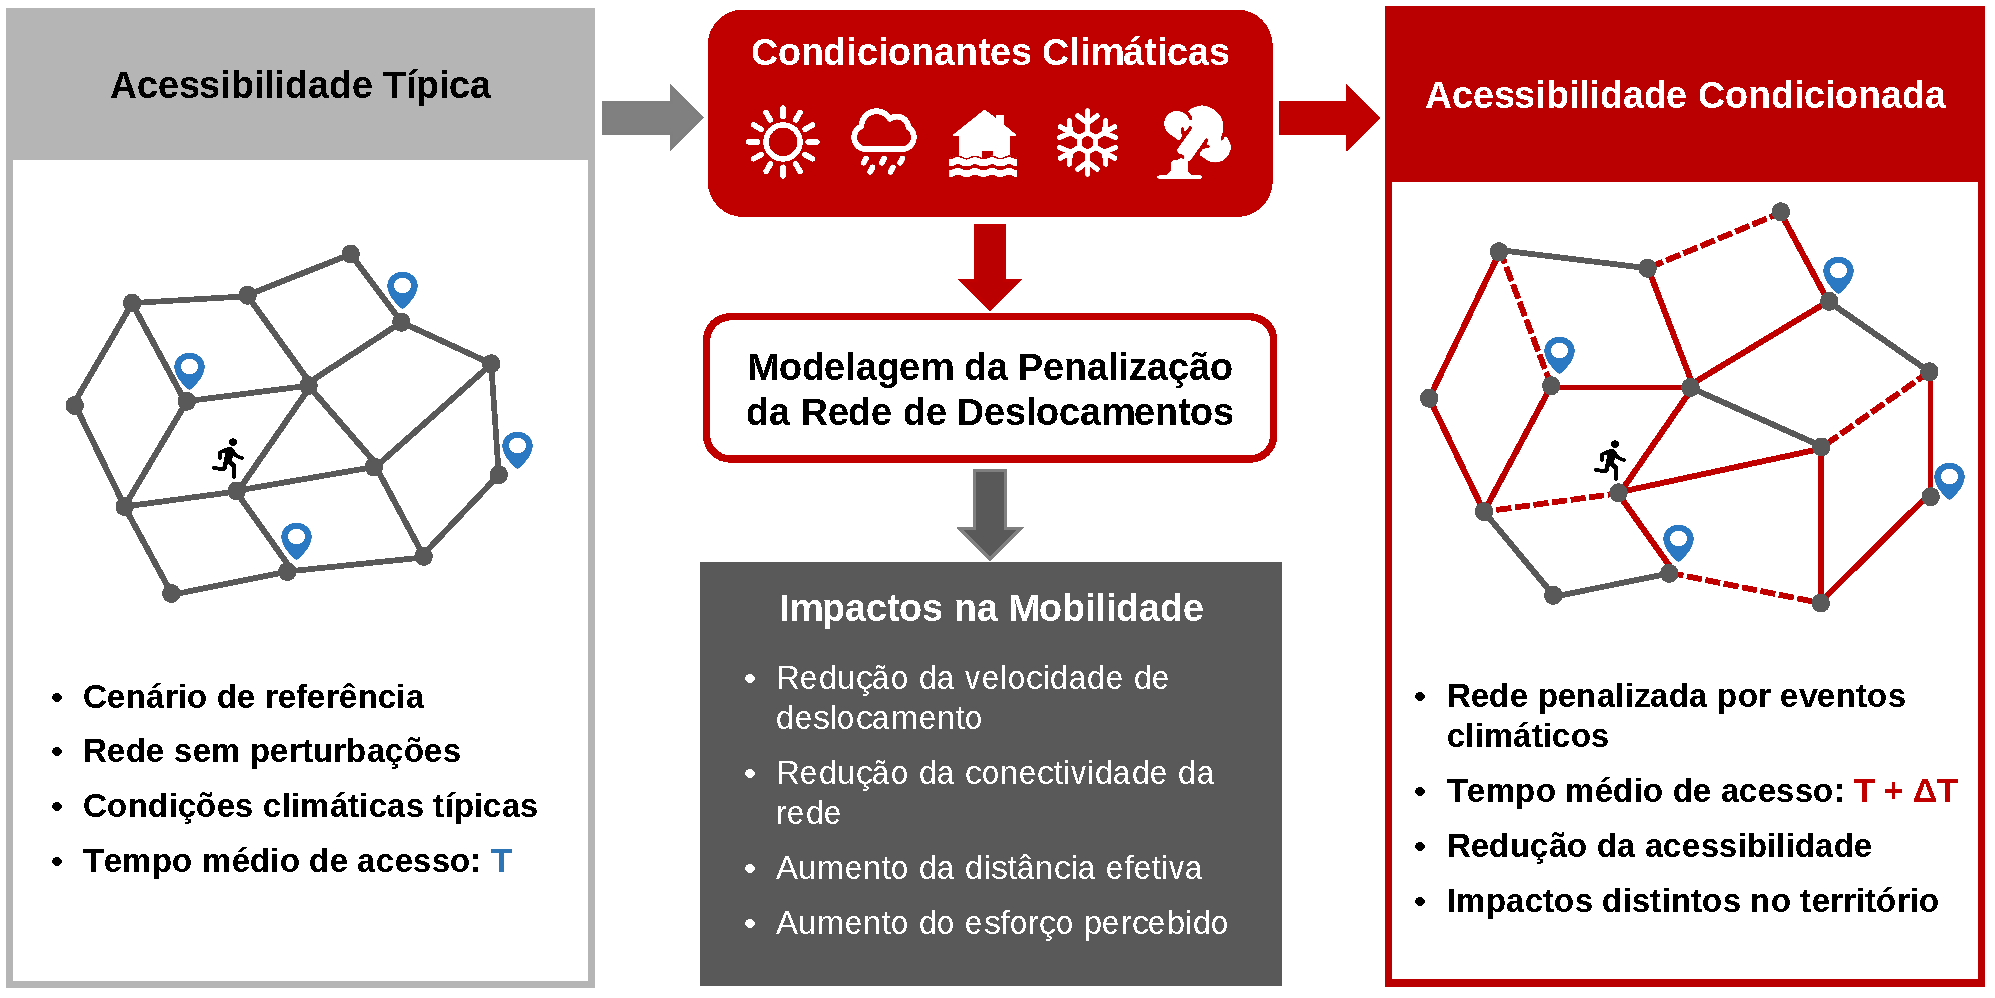
\includegraphics[width=1\textwidth]{figs/framework.pdf}
  \caption{Modeling flow for accessibility scenarios. Edges lengthen as their travel cost increases, so the geometry in the right panel encodes the effect of the disruption rather than the physical street layout.}
  \label{fig:framework}
\end{figure}

\subsubsection{Territorial Modeling}
\label{subsec:territorial_modelling}

The urban territory is assembled from four data types that differ in geometry, resolution, and coordinate reference system, and whose integration is the first source of complexity in the pipeline.

\begin{description}
  \item[Analysis grid.] A regular partition of the territory defining the minimum unit of study. The library supports hexagonal and square cells; the side or radius is a parameter set according to the transport mode and the local context. With hexagonal cells, the distance between neighboring centroids is uniform in all six directions, which avoids the directional bias that square cells introduce in neighborhood-based aggregation. The centroid of each cell is the theoretical origin of trips and the basis for computing and aggregating indicators.
  \item[Points of interest (POIs).] The destinations of trips: coordinates locating the everyday services used by the population, organized into categories such as health, education, and transport. Their selection depends on the availability of local databases, whether official or crowdsourced. Each POI is snapped to the nearest network vertex before routing, so the reachable set is bounded by the network rather than by straight-line distance.
  \item[Street network.] The mobility infrastructure is structured as a spatial graph, with vertices at intersections and edges along street segments whose initial base weight is travel time. Each cell centroid is attached to the nearest network vertex, and a maximum snap distance discards cells whose centroid lies too far from the network — a parameter that prevents a cell in an unmapped area from being routed through a vertex several kilometers away. Because this threshold removes cells from the analysis, it must be reported alongside the results.
  \item[Environmental layers.] Spatial layers that may be continuous, such as raster images, or discrete, such as vector polygons, mapping the climate or environmental phenomena under evaluation. A single scenario may stack several such layers. They are overlaid on the street network to adjust the travel cost of affected edges, as described in Section~\ref{sec:penalization}.
\end{description}

A fifth input completes the model. \textbf{Demographic and socioeconomic data} characterize the resident population — density, income, and schooling — and come from official censuses. These data are published in irregular administrative units such as census tracts, which do not align with the analysis grid, so each tract attribute is transferred to the cells by area-weighted mean: a cell receives the average of the tract values covering it, weighted by the intersected area. Where a tract has no value, its area is excluded from the denominator, so a cell partially covered by suppressed data is not diluted toward zero. The numerator and denominator are both taken from tracts with data, which keeps the cell value equal to the value of its contributing tracts rather than to a fraction of it.

This distinction between interpolation by density and aggregation by area is not interchangeable. Density interpolation conserves totals and suits population counts; area-weighted averaging preserves the value of the attribute itself and suits rates and indices. Population is interpolated the first way, socioeconomic indices the second.

\subsection{The Cost-Modification Mechanism}
\label{sec:penalization}

The framework fixes neither which environmental variables alter the network nor the magnitude of their effect. It exposes a \emph{mechanism} that receives environmental layers and returns a new cost for each edge; selecting the layers and setting their parameters belongs to whoever applies the method. This section describes that mechanism.

\subsubsection{Scenarios}

The network is evaluated in two states. In the \textbf{typical scenario}, each edge weight ($W_{base}$) is the travel cost under normal conditions — the segment length divided by the mean speed adopted for the mode under analysis. In the \textbf{conditioned scenario}, weights are recomputed from the environmental layers ($C$), producing $W_{cond}$ for each edge.

Comparing the two states isolates the effect of the disruption: any difference in accessibility indicators is attributed to the cost change introduced by the environmental layers.

\subsubsection{Cost modifiers}

The core element of the mechanism is the \emph{cost modifier}. Each modifier is a function that takes the value of a layer at a point on the edge and returns a multiplicative factor:

\begin{equation}
  f(v) \rightarrow \mathbb{R}^{+}
\end{equation}

where $v$ is the value sampled from the layer at that point. The factor $f$ may exceed 1 (penalization), fall below 1 (attenuation), or be infinite (interdiction). The same mechanism covers all three cases, which is why the framework refers to \emph{cost modifiers} rather than penalties alone.

A modifier never receives the whole edge: it is applied to values sampled along it. Sampling strategy and factor aggregation are declared separately, so phenomena with different spatial distributions are handled by the same mechanism.

\subsubsection{Sampling}

Two sampling strategies are available, and the choice trades cost for fidelity. \textbf{Midpoint} queries the layer at the edge midpoint and applies a single factor to the entire edge, which is fast but inaccurate when the edge crosses a boundary. \textbf{Segments} places $n$ equidistant points along the edge, including both endpoints, and reads the layer at each; the value of $n$ is a parameter, defaulting to four.

The distinction matters most for long edges, which are common in peripheries where blocks are large. A single edge can span several hundred meters and cross more than one thermal or topographic zone. Sampling only its midpoint may place the entire segment in the wrong class.

\subsubsection{Reading the layers}

How a layer is queried depends on the nature of the data.

\textbf{Continuous data} (rasters) are sampled at the chosen points. Each point takes the value of the pixel containing it. Points landing on a nodata pixel leave the cost unchanged at that location rather than propagating a missing value into the cost, so an incomplete raster degrades coverage instead of corrupting the network.

\textbf{Discrete data} (vector polygons) are queried by intersection. The edge is partitioned at every point where a polygon boundary crosses it, and each resulting sub-segment receives the factor of the polygon covering it. Sub-segments outside any polygon keep the original cost. Where polygons overlap, the \emph{largest} factor among them applies to the overlap, so a region mapped by two hazard layers is governed by the more restrictive one.

\subsubsection{Aggregation and interdiction}

The factors obtained along an edge must be reduced to a single value for the whole edge. The framework offers two reductions:

\begin{itemize}
  \item \textbf{Maximum}: adopts the most restrictive factor observed along the segment, treating the edge by its worst case. This is conservative and appropriate when the sample is small.
  \item \textbf{Length-weighted mean}: each sub-segment pays its own factor, and the mean is weighted by extent. This is more faithful on long edges crossing heterogeneous regions.
\end{itemize}

Infinite factors receive separate treatment. Assigning $f = \infty$ to a sub-segment declares it impassable: the cost of any path crossing it becomes infinite, and routing prefers alternatives. Interdiction is not a high cost but a statement that crossing is not viable in that scenario — the appropriate treatment for phenomena that block the road rather than delay it, such as a landslide burying the segment. When no alternative exists, the cell reaches no destination at all, a situation recorded as access loss.

\subsubsection{Composition}

When more than one environmental layer affects the same edge, modifiers are applied in sequence and the result accumulates multiplicatively:

\begin{equation}
  W_{cond} = W_{base} \times f_1 \times f_2 \times \cdots \times f_n
\end{equation}

Each step receives the cost produced by the previous one. Because multiplication commutes, the order does not change the numeric result, but it changes how the process reads, which matters when attributing an accessibility change to a specific layer.

This composition admits two arrangements. In \emph{simple rules}, each modifier queries one layer independently and chaining happens across rules. In \emph{composite rules}, several layers are queried at the same point on the edge and the factor is computed jointly, allowing one layer's effect to depend on another's value.

The distinction is not cosmetic. In the simple arrangement, an attenuation by vegetation would apply to any tree-lined segment, including where there is no heat at all — dense canopy next to a shaded, cool street would still receive a discount. In the composite arrangement, vegetation attenuates only where the thermal layer exceeds a threshold at that same point, so the two factors are evaluated jointly rather than independently averaged. A composite rule thus samples all its layers at identical locations before aggregating, preserving the spatial correspondence between their values.

\subsubsection{Recalculation and indicators}

With conditioned costs defined, a least-cost path algorithm runs over the graph, producing travel-time matrices for both scenarios. From these, the indicators described in Section~\ref{subsec:territorial_modelling} are computed: the mean time to reach the $k$ nearest POIs of each category (PTh), the inequality of its distribution (index G), and the share of the population served within a threshold (F15).

The scenario comparison adds per-cell time variation and \emph{access loss}: cells reaching no POI under the conditioned scenario receive infinite time and are accounted for separately. They are not an extreme case of high time but the absence of access, and treating them as a numeric value would distort any mean or inequality index computed over the remainder.

\subsection{Applicability}
\label{subsec:applicability}

This section states the criterion by which the scenarios were selected. The mechanism must handle environmental evidence in several forms, and each scenario instantiates one of them.

\subsubsection{Selection Criterion}

The mechanism varies along three axes: whether the environmental layer is continuous or discrete, whether several layers are read independently or jointly at the same location, and whether the effect is a penalization or an interdiction. Each scenario instantiates one combination of these values, and the set was chosen so that each axis appears at both of its values.

Several scenarios run on the same city and differ only in the layers they declare, so the variation in behavior follows from configuration.

\subsubsection{Coverage of the Mechanism}

Table~\ref{tab:cenarios} lists the seven conditioned scenarios by the capability each exercises.

\begin{table}[H]
\centering
\footnotesize
\caption{Scenarios by the capability of the mechanism they exercise}
\label{tab:cenarios}
\begin{tabularx}{\linewidth}{|l|l|X|l|}
\hline
\textbf{Scenario} & \textbf{Layers} & \textbf{Capability exercised} & \textbf{Effect} \\
\hline
\texttt{thermal} & 1 raster & Sampling of a continuous field & penalization \\
\texttt{thermal+green} & 2 rasters, joint & Composite rule over co-located layers & penalization \\
\texttt{thermal\_demo} & 1 raster & Response to a steeper gradient & penalization \\
\texttt{thermal+green\_demo} & 2 rasters, joint & Composite rule under a steeper gradient & penalization \\
\texttt{flood} & 1 vector & Partition at polygon boundaries & penalization \\
\texttt{landslide} & 1 vector & Same, with infinite factors & interdiction \\
\texttt{flood+landslide} & 2 vectors & Sequential composition, interdiction dominates & both \\
\hline
\end{tabularx}
\end{table}

Three properties follow from the table.

\textbf{Both branches of the modifier are exercised.} Curitiba samples continuous fields and Porto Alegre intersects polygon geometries, which are distinct implementation paths.

\textbf{Both outcomes of the cost function are exercised.} Flooding raises travel cost while preserving every connection, so all paths exist in both scenarios with a different weight. Landsliding makes segments impassable, and some origins lose access entirely. The framework reports the second separately, since it is an absence of access and not a slowdown.

\textbf{Composition appears in homogeneous and sequential form.} The \texttt{thermal+green} scenario reads two rasters at identical sampled points and returns a single factor, the thermal one multiplied by the shading reduction wherever vegetation is present. Sampling both layers at the same position is what requires a composite rule: two chained simple rules would each sample the segment independently and could read vegetation at a point whose temperature was read elsewhere. The \texttt{flood+landslide} scenario applies two vector rules in sequence, and the interdiction of one dominates the penalization of the other on shared edges.

\subsubsection{Demonstrative Scenarios}

Two Curitiba scenarios use a thermal coefficient roughly seven times the calibrated value. They are demonstrative, and the text does not read them as estimates. Their purpose is to show that the mechanism responds monotonically to the magnitude of its input: a steeper gradient that produced a smaller accessibility change would indicate a defect in the composition. Reporting them alongside the calibrated scenarios makes the sensitivity of the pipeline observable at no additional cost, since they differ only in a parameter.
\subsubsection{Scope and Limitations}

Two limits follow from the design and belong alongside the results.

\textbf{The mixed representation is supported at the component level.} The implementation reads a raster and a vector at the same sample point, and tests cover this path, but no scenario here declares one of each. Doing so requires a study area where both evidence types describe the same phenomenon, which the two municipalities do not provide.

\textbf{The estimates await validation against observations.} Accessibility under a hypothetical disruption has no measured counterpart, since the conditioned scenario did not occur. This work establishes that the mechanism computes what it specifies and that the framework accommodates disruptions of different forms. Matching the resulting travel times to what pedestrians would experience requires observed mobility under an actual event.

Together these limits place the contribution: a framework demonstrated to be applicable across representations and outcomes. Empirical validation of its predictions remains open.


\section{Case Studies}
\label{sec:case_studies}

The framework was applied to two Brazilian state capitals, Curitiba (PR) and Porto Alegre (RS). The two cities instantiate the two environmental representations supported by the mechanism: Curitiba carries a continuous field, a surface temperature raster, while Porto Alegre carries discrete polygons delimiting areas at geological risk. Both cities are covered by OpenStreetMap with sufficient completeness for pedestrian routing, both are served by census tracts from the same national survey, and their environmental layers are published by official agencies in open formats. The cases therefore share the data model and differ in the environmental evidence they declare, which is the condition under which the comparison between them is meaningful.

\subsection{Cases and shared configuration}
\label{subsec:shared-config}

Table~\ref{tab:shared-config} lists the parameters held fixed across both cities. Fixing them is what allows an observed difference in accessibility to be attributed to the environmental layer rather than to the computational setup.

\begin{table}[htbp]
\centering
\caption{Parameters held fixed across both case studies.}
\label{tab:shared-config}
\begin{tabular}{lll}
\hline
Parameter & Value & Effect on the analysis \\
\hline
Grid geometry & hexagonal & no directional bias in distance \\
Cell size & 200 m radius & $\approx 0.104$ km$^2$ per cell \\
Network type & walkable & pedestrian graph only \\
Walking speed & 5.0 km/h & converts length to travel time \\
Nearest POIs ($k$) & 3 & PTh averages the three closest \\
Maximum snapping & 200 m & cells farther from the graph are discarded \\
POI buffer & 2000 m & bounds the reachable set \\
POI source & OpenStreetMap & same extraction rule in both cities \\
Socioeconomic source & Census 2022 & same variables and aggregation \\
\hline
\end{tabular}
\end{table}

The travel time of an edge is its length divided by the walking speed, which is held constant so that a change in cost reflects the environmental factor alone. Each cell is attached to the nearest network node, and cells whose centroid lies farther than 200 m from any node are discarded rather than assigned to a distant one. The threshold retains 3{,}855 cells in Curitiba and 3{,}065 in Porto Alegre. What it removes is demographically marginal: the discarded cells hold 0.7\% of the population in Curitiba and 1.6\% in Porto Alegre, so the analysis covers 99.3\% and 98.1\% of the resident population respectively. The excluded cells are those over water, parks, steep slopes and vacant land, where there is no pedestrian network to attach to.

\subsection{Curitiba: a continuous conditioning variable}
\label{subsec:curitiba}

Curitiba is the case in which thermal discomfort acts as a continuous modifier of walking effort. The conditioning layer is a land surface temperature (LST) composite derived from Landsat 8 and 9 imagery, Thermal Infrared Sensor, band \texttt{ST\_TRAD}. The layer is an annual median, which suppresses cloud contamination and isolates the persistent spatial pattern from the day-to-day variation that would make a single scene unrepresentative.

Land cover is the second layer. The source is the 2019 vegetation inventory published by the Instituto de Pesquisa e Planejamento Urbano de Curitiba (IPPUC), distributed as roughly 126 thousand fragmented polygons. Because sidewalks run around squares and parks rather than through them, only 3.4\% of the network's sampled points fell inside a vegetation polygon, and the layer would have had no measurable effect. The vector source is therefore rasterized to a binary 5 m grid and dilated by 5 m, the crown radius of a mature street tree, which models the shade cast onto the adjacent sidewalk and raises coverage to 24.1\% of the network.

The thermal factor follows a linear form, $f(T) = \max\left(1 + k\,(T - t_0),\, 1\right)$, with $k = 0.0070$~°C$^{-1}$ and $t_0 = 23$~°C. The slope derives from the 7\% reduction in economical walking speed measured between 23~°C and 33~°C~\cite{Horiuchi2018Economical}; $t_0$ is the thermoneutral reference of that study. The surface temperature of the composite ranges from 12.9~°C to 38.2~°C, with a median of 27.5~°C, so the factor spans 1.00 to 1.11 across the city. The lower bound holds 1 rather than rewarding cool pixels, since the source measures loss of speed under heat and not a gain under cold.

Vegetation multiplies the thermal factor by $0.958$, derived from a measured reduction of up to 3~s per 100~m in perceived travel time under street trees~\cite{Jia2023GreeningWalk}. At 5~km/h, 100~m take 72~s, and 69~s is 0.958 of that. The reduction applies wherever vegetation exists, including the cool parts of the city, because the source measures the effect on total travel time rather than on the thermal excess. A shaded street at 20~°C therefore receives a factor of $0.958$, below unity.

Reading the two layers at the same point requires a composite rule rather than two chained rules. Each simple rule samples the edge independently, so a segment sampled at four positions would take its temperature from one set of positions and its vegetation from another. The composite rule samples both layers at identical points and returns their product, which keeps the temperature and the shade that are actually at the same place.

\subsection{Porto Alegre: a discrete conditioning variable}
\label{subsec:porto-alegre}

Porto Alegre is the case in which the conditioning phenomenon is mapped as discrete polygons. Two layers are used, both produced by the Geological Survey of Brazil (SGB/CPRM) as a municipal geological risk zoning~\cite{Bellettini2022RiscoPOA} and distributed through the GeoPOA portal of the city administration: flood-prone areas (2,216 polygons, 250.8~km$^2$) and landslide areas (305 polygons, 76.4~km$^2$). Each polygon is classified as \textit{Alta}, \textit{Média} or \textit{Baixa}, a grading of risk that carries no water depth.

The two hazards call for different treatments, because they act on walking differently. Flooding delays the pedestrian without preventing passage, so its factor is finite and derived from measured speeds. The three classes are read as equivalents of the three depths tested by Li et al.~\cite{Li2026WaterDepth}, in ascending order of severity, and the factor of each class is the ratio between walking speed on dry ground and speed under that depth. This mapping is an assumption of the present application. It yields 1.71 for \textit{Baixa} (0.35~m), 1.86 for \textit{Média} (0.60~m) and 2.14 for \textit{Alta} (0.90~m), all computed from the mean speeds of the study's full sample.

A landslide leaves no passable road behind, and the literature offers no speed to calibrate against. The scenario therefore assumes the event has occurred and treats the landslide as an interruption, assigning an infinite factor to the \textit{Alta} and \textit{Média} classes and removing those edges from the graph.

\subsection{Socioeconomic layer}
\label{subsec:socioeconomic-layer}

Both cities are described by census tracts from the 2022 Brazilian Demographic Census. Tract variables are transferred to grid cells by area-weighted mean, and tracts that do not intersect a cell are excluded from the denominator rather than counted as zero.

Comparing accessibility between scenarios says how much access is lost, but not who loses it. To place the two against each other, each cell receives a socioeconomic deprivation index (SDI) built from three census variables, one per axis of stratification. The index is computed at the tract and only then carried to the cells, so that a share comes from the tract totals rather than from the average of area-weighted shares. Each axis is normalized within the city by its 2nd and 98th percentiles, which limits the influence of extreme tracts, and the three receive equal weight. All three are oriented so that a higher value means greater deprivation.

The first axis is the share of households without adequate sanitation, taken as the complement of the fraction served by a public sewer network or by a septic tank connected to it, and log-scaled because most tracts sit at or near zero and a few concentrate the deficit. The second is per capita income declared in the tract, taken as a logarithm because its distribution is strongly asymmetric and inverted so that lower income raises the index. The third is the illiteracy rate among heads of household, also log-scaled; schooling in years of study is not published at the tract level for the 2022 census, so literacy is the available proxy for educational condition.

\subsection{Socioeconomic analysis}
\label{subsec:socioeconomic-analysis}

The index measures the social condition against which the accessibility change is read. Three analyses are applied to each city and scenario, and they answer different questions.

Spearman correlations between each axis and the median per-cell increase in travel time test whether the axes are associated with the change at all. The coefficient is rank-based, so the association does not depend on the shape of either distribution — a property the axes need, since all three are skewed. The three axes are carried separately so that an association with one is not diluted by the other two.

An ordinary least squares regression with the three axes as simultaneous predictors estimates how much of the variation each one accounts for once the others are held. Correlated axes produce similar marginal correlations but different partial coefficients, and the regression separates them. The dependent variable is again the median increase per cell, and the reported quantities are the coefficient, its standard error, and the model's adjusted coefficient of determination.

Correlation and regression treat cells as independent observations, which they are not: neighbouring cells share conditions, infrastructure and environmental exposure. A bivariate Moran's I with a queen contiguity matrix measures whether the association between an axis and the accessibility change is spatially organized, and the local indicator identifies where. Significance comes from 999 permutations, and each cell is classified into the four quadrants — high axis with high change, low with high, low with low, high with low — according to the quadrant in which the local statistic falls. This separates an association spread across the city from one confined to particular areas, which aggregate coefficients cannot show.

\subsection{Scope of the comparison}
\label{subsec:scope-comparison}

The two cities share the extraction rule for points of interest, the routing parameters and the indicator definitions, so a difference in their accessibility indicators reflects a difference in their territories and in their environmental layers. The coverage of the underlying crowdsourced map is not uniform, however. Curitiba contributes 975 public transport stop positions to the point set, against 121 in Porto Alegre, and this asymmetry propagates to the transportation category, which holds 1,012 points in Curitiba and 170 in Porto Alegre. Indicators for the remaining categories rest on comparable point counts. The transportation results are reported, but comparisons involving that category should be read with the mapping density of each city in mind rather than as a difference between the cities themselves.

\section{Resultados}
\label{sec:results}

Esta seção descreve os avanços já realizados na pesquisa, validados por meio de publicação científica, e detalha os resultados finais que se espera alcançar com a aplicação completa da metodologia proposta.

\subsection{Resultados Parciais}
Como prova de conceito da etapa de modelagem territorial e cálculo de indicadores, foi desenvolvido o estudo intitulado \textit{"Fatores Socioeconômicos e Desigualdade na Mobilidade de Curta Distância aos Serviços Urbanos de Curitiba"} \cite{sbbd_estendido}, apresentado no Apêndice~\ref{apendice:fatores_socioeconomicos}. O trabalho, focado em deslocamentos a pé, estruturou a rede viária e os Pontos de Interesse das categorias de alimentação, comércio, cultura, educação, saúde e transporte, e calculou métricas de acessibilidade como o PTh, PTc e F15 para o cenário típico.

Por meio de análise de regressão e clusterização espacial, o estudo cruzou os tempos de acesso com variáveis socioeconômicas. Os resultados mostraram que variáveis como escolaridade, empregabilidade e acesso à infraestrutura básica estão diretamente associadas a melhores tempos de acesso aos serviços urbanos em Curitiba. Áreas com maior concentração de pessoas com mais anos de estudo ou maior frequência ao ensino médio tendem a apresentar tempos de deslocamento mais baixos e acesso facilitado, enquanto regiões marcadas por maior vulnerabilidade social, como presença de jovens fora da escola e do trabalho, precariedade de água e esgoto, e moradias em condições inadequadas, registram deslocamentos mais longos. 

A análise espacial confirmou que os maiores tempos de acesso se concentram nos setores periféricos da cidade, ampliando desigualdades já presentes nos indicadores socioeconômicos. Além disso, o estudo também identificou casos pontuais de territórios (\textit{outliers}) com oferta de serviços acima da média do entorno imediato, assim como áreas mais próximas as regiões centrais em situação de exclusão devido à carência de infraestrutura urbana.

Embora o estudo tenha consolidado a coleta de dados e o cálculo base da acessibilidade, ele apresentou limitações que fundamentam o avanço metodológico desta dissertação. O modelo utilizou uma topologia estática, focando exclusivamente no cenário típico a pé, sem considerar barreiras físicas temporárias, perturbações ambientais ou a qualidade e capacidade de atendimento dos serviços.

\subsection{Resultados Esperados}

Com a aplicação integral da metodologia proposta, espera-se demonstrar de forma quantitativa como perturbações climáticas e ambientais podem degradar significativamente a acessibilidade urbana em comparação ao cenário típico. O trabalho deverá validar o mecanismo de penalização do grafo, mostrando na prática como a introdução de camadas ambientais altera o custo do deslocamento e modifica a topologia funcional da cidade. Os resultados esperados incluem a produção de mapas detalhados, capazes de identificar regiões que, embora tradicionalmente bem servidas de acessibilidade, se tornam isoladas ou apresentam forte degradação sob condições ambientais adversas.

Além disso, a análise irá quantificar os efeitos dessas perturbações sobre diferentes grupos sociais, por meio da aplicação de métricas como o Índice G e o cruzamento com indicadores socioeconômicos. Assim, será possível evidenciar se as perdas de acesso afetam a população de forma homogênea ou se recaem de maneira mais intensa sobre territórios e grupos em situação de vulnerabilidade. Espera-se, portanto, fornecer um panorama analítico robusto que possa subsidiar o planejamento urbano e orientar políticas públicas mais resilientes, considerando não apenas a oferta de oportunidades, mas também as barreiras dinâmicas impostas pelo clima e pelo ambiente ao acesso dos cidadãos.
\section{Discussão e Limitações}
\label{sec:discussion}

% A preencher.
%
% Pontos previstos:
% - LST != temperatura do ar: viés espacialmente sistemático (ver decisoes.md)
% - velocidade de caminhada calibrada em câmara, não em campo
% - modelo pressupõe manutenção do deslocamento a pé
% - indicadores medem potencial de acesso, não qualidade do serviço

\section{Conclusão}
\label{sec:conclusion}

% A preencher.


\bibliographystyle{sbc}
\bibliography{refs}

\newpage
\appendix
\pagestyle{empty}

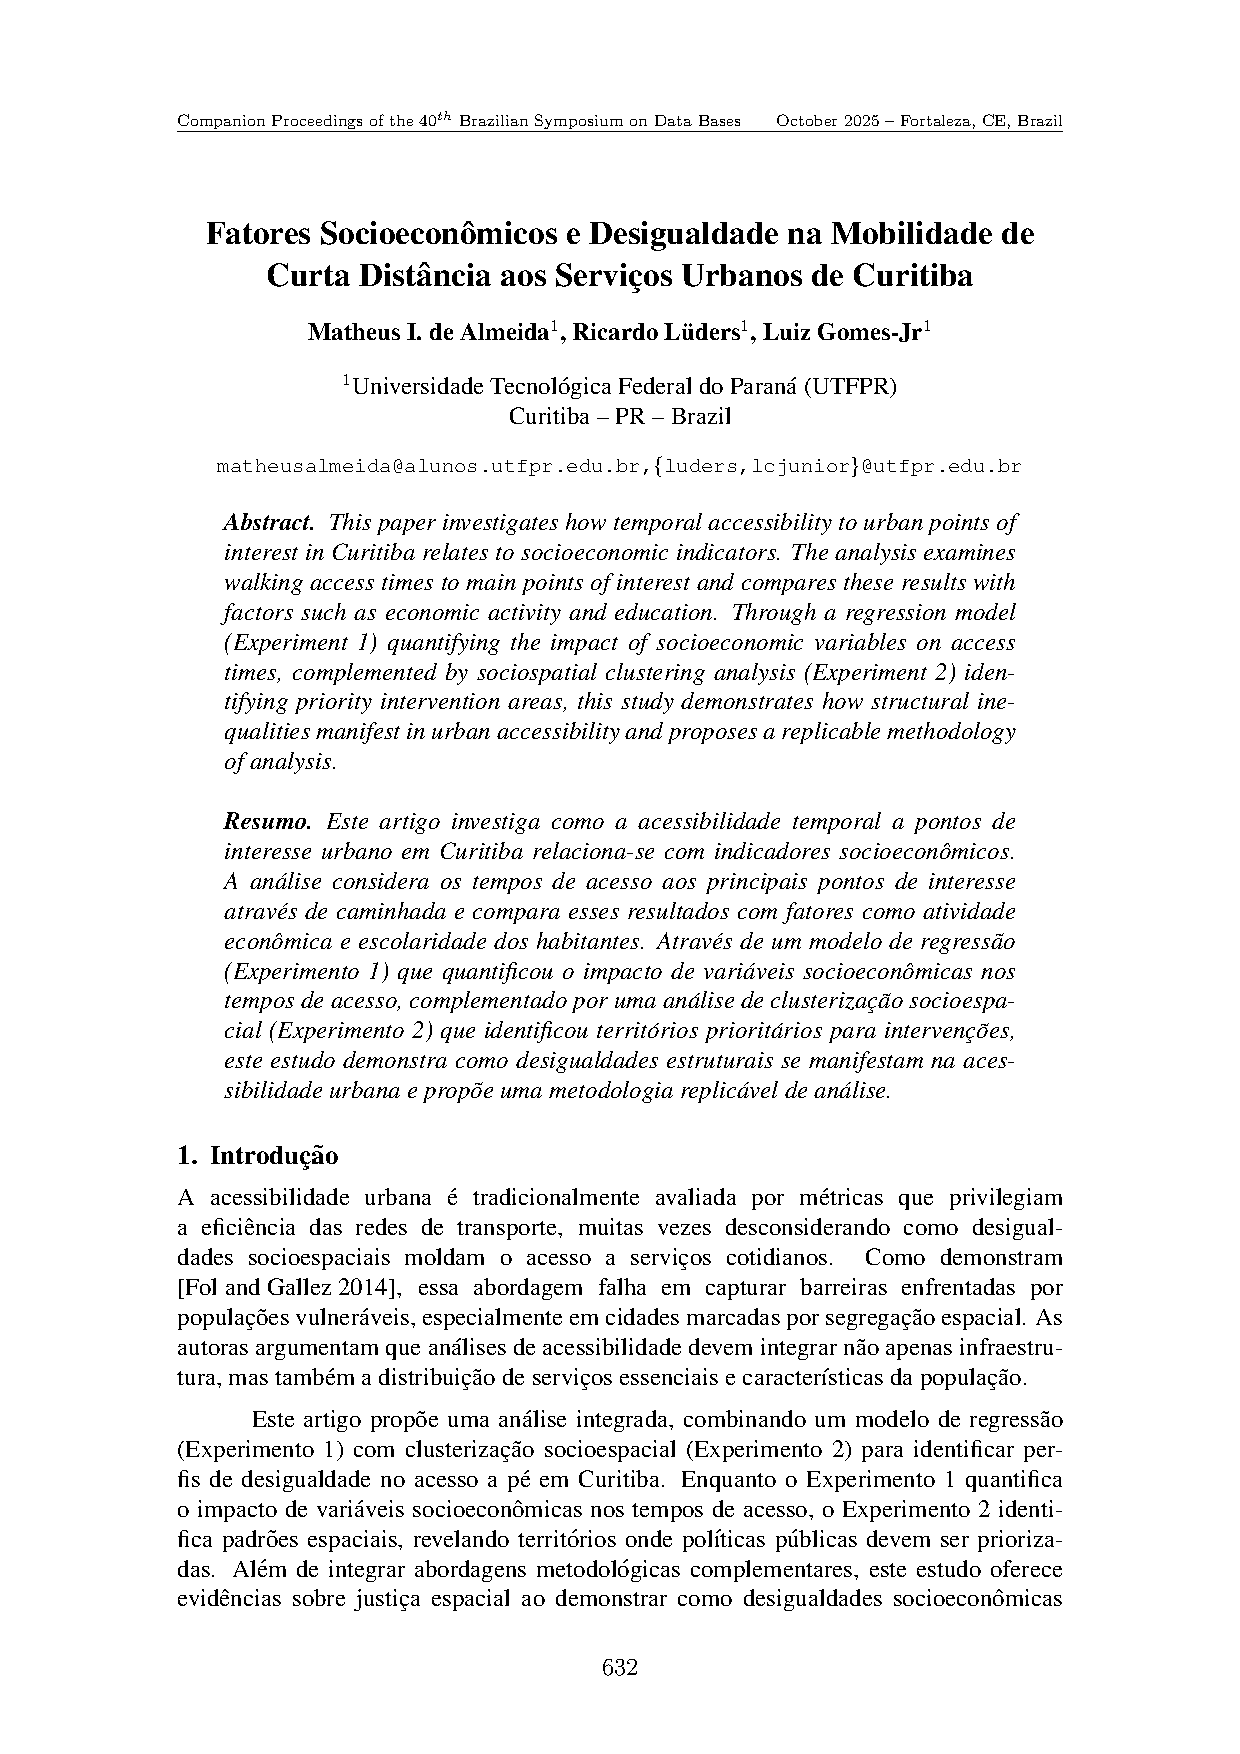
\includepdf[
    pages=1, 
    scale=0.8, 
    pagecommand={\section{Apêndice A}\label{apendice:fatores_socioeconomicos}}
]{files/fatores_socioeconomicos.pdf}

\includepdf[pages=2-, scale=0.9]{files/fatores_socioeconomicos.pdf}

\end{document}
